\documentclass[t,compress,mathserif,10pt,xcolor=dvipsnames, table, aspectratio=43]{beamer}

\usepackage[T1]{fontenc}
\usepackage[utf8]{inputenc}
\usepackage[frenchb]{babel}
\usepackage{eulervm}
\usepackage{etoolbox,refcount}

\usepackage[normalem]{ulem} %strikeout with \sout{}

%%%%% Colors
\definecolor{bleuUni}{RGB}{0, 157, 224}
\definecolor{marronUni}{RGB}{68, 58, 49}
\usecolortheme[named=bleuUni]{structure}
\input{colors}
%%%%%%%%%%%%%%%%%%%

%%%%% Tabs
\usepackage{booktabs}
\usepackage{multirow}
\usepackage{multicol}
\usepackage{makecell}
%\usepackage{enumitem}
%%%%%%%%%%%%%%%%%%%%


%%%%% Plots
\usepackage{pgfplots}
 \pgfplotsset{compat=newest}
 \usepgfplotslibrary{groupplots}
\usepackage{tikz}
  \usetikzlibrary{matrix, positioning, patterns, shapes, arrows, shapes.multipart, decorations.pathmorphing}
\usepackage{circuitikz}
\usepackage{tikz-timing}      % package pour les chronogrammes
\usepackage{caption}
\usepackage{graphicx}
\usepackage[export]{adjustbox} %align in includegraphics
\tikzset{
    invisible/.style={opacity=0},
    visible on/.style={alt={#1{}{invisible}}},
    alt/.code args={<#1>#2#3}{%
      \alt<#1>{\pgfkeysalso{#2}}{\pgfkeysalso{#3}} % \pgfkeysalso doesn't change the path
    },  
}
%%%%%%%%%%%%%%%%%%%%


%%%%% Algo
\usepackage[french,onelanguage, ruled, linesnumbered, vlined]{algorithm2e}
\SetAlFnt{\footnotesize}
%%%%%%%%%%%%%%%%%%%%


%%%%% Math
\usepackage{stmaryrd} %llbracket
\usepackage{amsmath}
\usepackage{amssymb}
\usepackage{marvosym} %grosse fleche
\usepackage{calc}
\DeclareMathOperator{\card}{card}
\DeclareMathOperator*{\maxstar}{max*}
\DeclareMathOperator*{\argmax}{arg\,max}
\DeclareMathOperator*{\decide}{decide}
\DecimalMathComma
%%%%%%%%%%%%%%%%%%%%


%%%%%% Special commands : ddfrac and actionenv and compresslist

\newcommand\ddfrac[2]{\frac{\displaystyle #1}{\displaystyle #2}}

\newenvironment<>{varblock}[2][\textwidth]{%
  \setlength{\textwidth}{#1}
  \begin{actionenv}#3%
    \def\insertblocktitle{#2}%
    \par%
    \usebeamertemplate{block begin}}
  {\par%
    \usebeamertemplate{block end}%
  \end{actionenv}}

\newcommand{\compresslist}{ % Define a command to reduce spacing within itemize/enumerate environments, this is used right after \begin{itemize} or \begin{enumerate}
\setlength{\itemsep}{1pt}
\setlength{\parskip}{0pt}
\setlength{\parsep}{0pt}
}

\newcommand*\circled[1]{\tikz[baseline=(char.base)]{%
      \node[shape=circle,fill=bleuUni,inner sep=2pt] (char) {\textbf{\textcolor{white}{#1}}};}}

\newcommand{\itmsp}[1] {\setlength\itemsep{#1}}
%%%%%%%%%%%%%%%%%%%%%%%%%


%%%%% Beamer
\usepackage[bars]{beamerthemetree} % Beamer theme v 2.2
\mode<presentation>
\newcommand*\oldmacro{}%
\let\oldmacro\insertshorttitle%
\renewcommand*\insertshorttitle{%
 \oldmacro\hfill%
\insertframenumber\,/\,\inserttotalframenumber}
\setbeamertemplate{footline}[frame number]
\setbeamersize{text margin left=10pt,text margin right=10pt}
\setbeamerfont{frametitle}{size=\small}
\setbeamertemplate{frametitle}{ \nointerlineskip %
\begin{beamercolorbox}[wd=\paperwidth,ht=2.2ex,dp=.9ex,left]{frametitle} %
                       \hspace*{2ex}\strut\bfseries\color{bleuUni!15!white}\insertframetitle\strut\par %
\end{beamercolorbox}}

%\setbeamerfont{headline}{size=\footnotesize}

% \usepackage{animate}
% \usepackage{multimedia}
\usetheme{Ilmenau} % Beamer theme v 3.0
\setbeamercolor{section in head/foot}{bg=marronUni}
\useinnertheme{circles} %rectangle bullet points instead of circle ones
\usepackage{beamerthemebars}
\beamertemplatenavigationsymbolsempty
%\setbeamercolor{navigation symbols dimmed}{fg=red!80!black}
%\setbeamercolor{navigation symbols}{fg=red!80!black}
%%%%%%%%%%%%%%%%%%%%%%%%%

\setbeamertemplate{headline}{%
\begin{beamercolorbox}[colsep=1.5pt]{upper separation line head}
\end{beamercolorbox}
\begin{beamercolorbox}{section in head/foot}
    \vskip2pt\insertsectionnavigationhorizontal{\paperwidth}{}{}\vskip2pt
\end{beamercolorbox}%
\begin{beamercolorbox}[ht=10pt]{subsection in head/foot}%
    \vskip2pt\insertsubsectionnavigationhorizontal{\paperwidth}{}{}\vskip2pt
\end{beamercolorbox}%
\begin{beamercolorbox}[colsep=1.5pt]{lower separation line head}
\end{beamercolorbox}
}

\setbeamertemplate{blocks}[rounded][shadow=true]



%%%%% Title
\title{\textbf{Contributions à l'amélioration des \\%
               performances de décodage des turbo codes : \\%
               algorithmes et architecture}}
%\subtitle{algorithms et arhitecture}\hspace{10.7cm}
\author[Thibaud Tonnellier\hspace{7.51cm}{thibaud.tonnellier@ims-bordeaux.fr}]    {Thibaud Tonnellier}
\titlegraphic{
\includegraphics[height=.7cm]{logos/ims.png} \hfil %
              
\includegraphics[height=.7cm]{logos/inp.PNG} \hfil %
              
\includegraphics[height=.7cm]{logos/ub.png}  \hfil %
              
\includegraphics[height=.7cm]{logos/tas.png}}
%\pgfdeclareimage[height=.8cm]{le-logo}{logo.png}
%\logo{\pgfuseimage{le-logo}\hspace{\dimexpr\paperwidth-1.55cm}\vspace{-8pt}}
%%%%%%%%%%%%%%%%%%%%%%%%%


%%%%% Contents each new sec and subsec
\AtBeginSection[]
{
  \ifnumcomp{\value{section}}{=}{1}{}{
    \begin{frame}[c]{Plan}
      \centering
      \tableofcontents[
          currentsection,
          hideothersubsections
          %subsectionstyle=show/hide
      ]
    \end{frame}
  }
}

\AtBeginSubsection[]
{
  \begin{frame}[c]{Plan}
    \tableofcontents[
      currentsection,
      sectionstyle=show/shaded,
      subsectionstyle=show/shaded/hide
    ]
  \end{frame}
}

%%%%%%%%%%%%%%%%%%%%%%%%%%%%%%%%%%%%%%%%%%%%%%%%%%%%%%%%%%%%%%%%%%%%%%%%%%%%%%%%
\begin{document}

\begin{frame}[c]
  \titlepage
\end{frame}

%%%%%%%%%%%%%%%%%%%%%%%%%%%%%%%%%%%%%%%%%%%%%%%%%%%%%%%%%%%%%%%%%%%%%%%%%%%%%%%%
\section[]{Contexte}
\begin{frame}[c]
  \begin{block}{Problématique industrielle}
    $\color{bleuUni}\bullet$ Un standard de communication fixe un protocole pour la transmission de l'information.\\
    $\color{bleuUni}\bullet$ Or, les besoins applicatifs peuvent évoluer et ne plus correspondre à ceux définis.\\
    $\color{bleuUni}\bullet$ Objectif : Améliorer les performances de transmissions sans modifier le codage et donc le standard.
 \end{block}
\end{frame}

\begin{frame}[c]
\centering
  Slide ctx 2
\end{frame}

\begin{frame}[c]
  \tableofcontents[ 
      subsectionstyle=hide,
  ]
\end{frame}

%%%%%%%%%%%%%%%%%%%%%%%%%%%%%%%%%%%%%%%%%%%%%%%%%%%%%%%%%%%%%%%%%%%%%%%%%%%%%%%%
\section[Introduction]{Introduction et problématique} 

%%%%%%%%%%%%%%%%%%%%%%%%%%%%%%%%%%%%%%%%
\subsection{Le codage de canal}
\begin{frame}[c]{Chaîne de communication numérique} 
    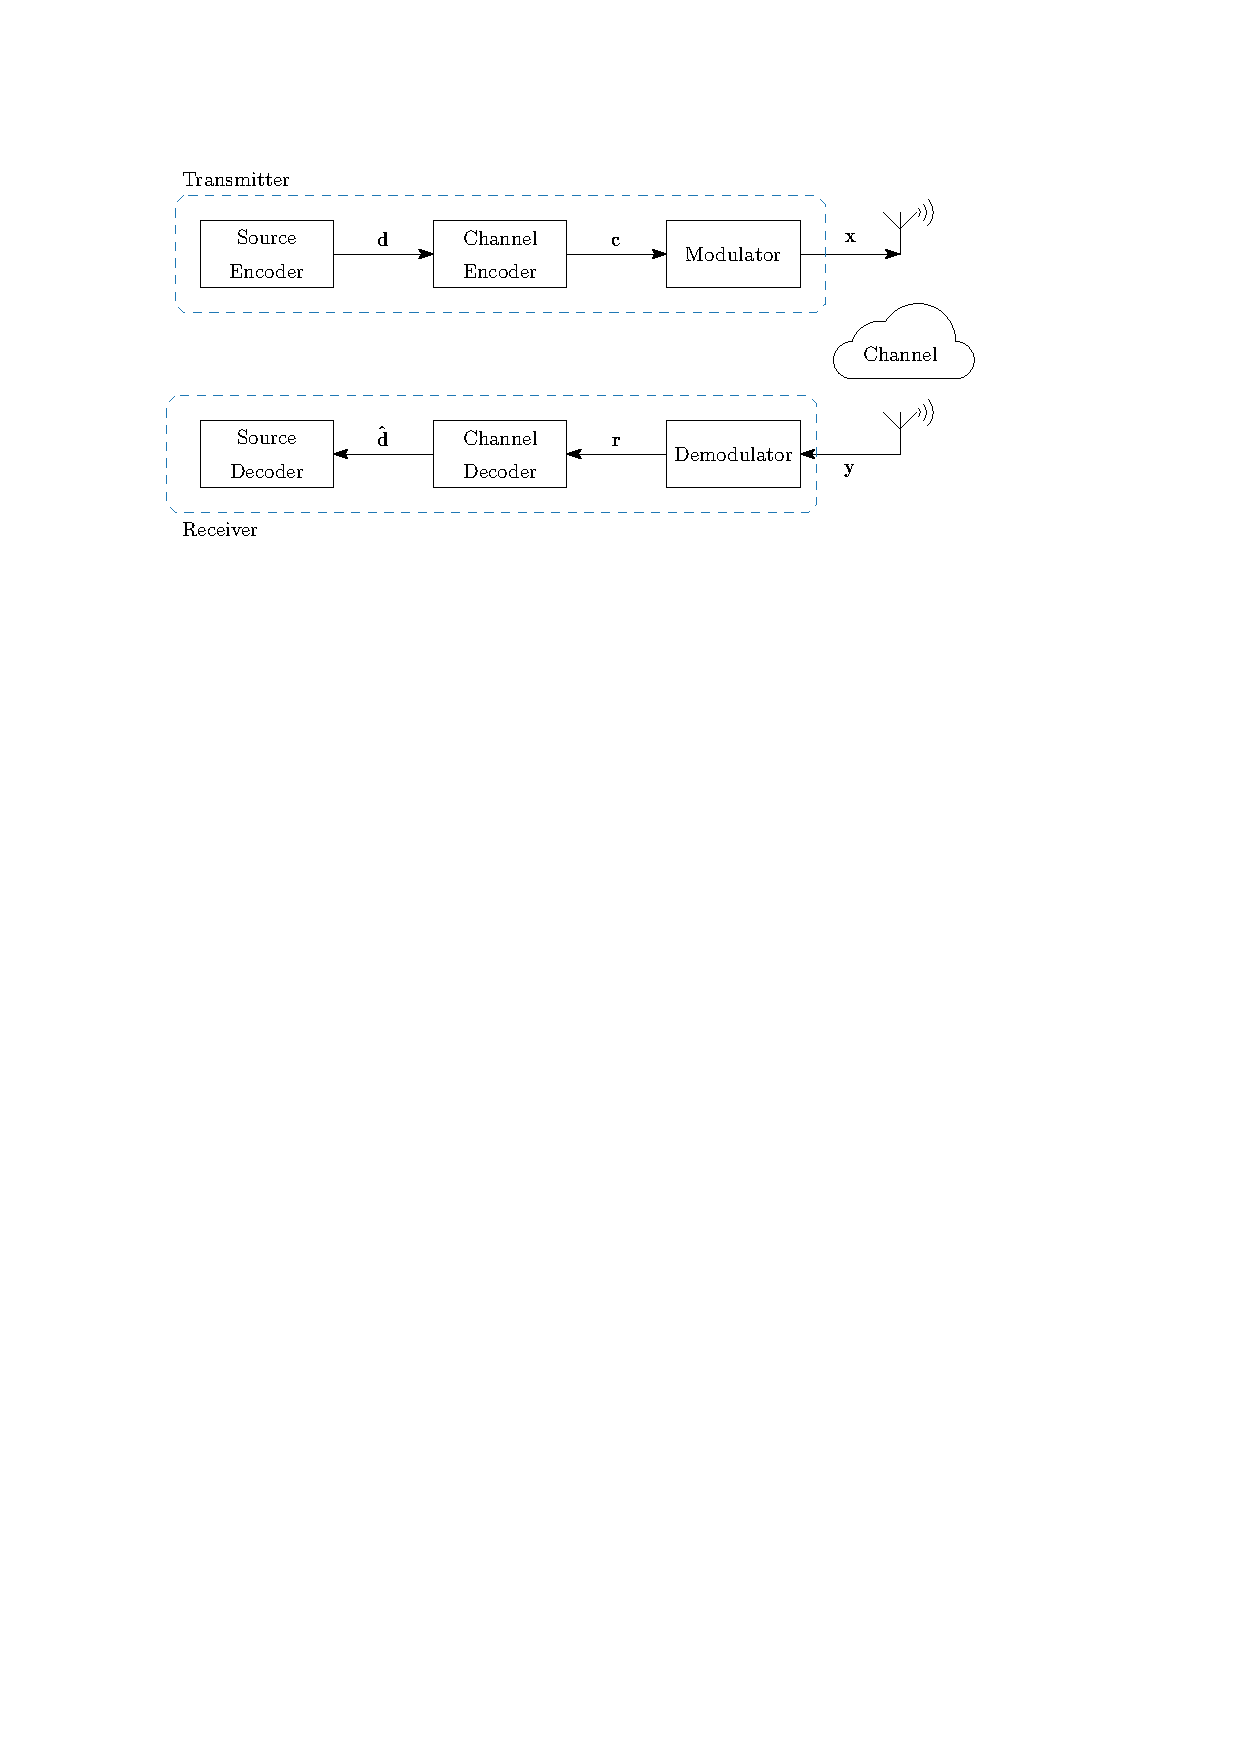
\includegraphics[width=0.7\textwidth, center,page=1]{fig/shParadigm2.pdf}
    \vspace*{1ex}
    \begin{itemize}\itmsp{1em}
      \item Codeur de source : obtenir le maximum de concision dans l’expression d'un message.
      \item Codeur de canal : rendre robuste un message face aux perturbations du canal. 
      \item Canal : Perturbations (ex : bruit, interférences...)
    \end{itemize}
\end{frame}

\begin{frame}[t]{Courbes de performances et limites}
\begin{center}
\only<1>{\vspace*{-1.1ex}}
\begin{tikzpicture}
  \begin{semilogyaxis}[footnotesize, width=0.9\linewidth, height=0.55\linewidth,    
      %xmin=-1, xmax=10, xtick={-1, 0,...,10},
      xmin=-1, xmax=9, xtick={-1, 0,...,9},
      ymin=2e-5,  ymax=0.11,
      xlabel=$E_b/N_0 \text{(dB)}$, 
      ylabel=\only<1>{Taux d'erreur binaire}\only<2->{Probabilité et taux d'erreurs binaires},
      grid=both, grid style={gray!30},
      tick align=outside, tickpos=left, % legend columns=2, legend style={at={(1, -.25), anchor=north}, /tikz/column 2/.style={column sep=5pt}} 
      ]

      \addplot[mark=none,Paired-5, semithick, visible on=<2->]  table [x=SNR, y=BER] {../main/ch1_fig/berBPSK.dat}; \label{bpsk}
      \addplot[mark=o,   Paired-1, semithick, visible on=<3->]  table [x=SNR, y=BER] {../main/ch1_fig/berRSC.dat};  \label{rsc}
      \addplot[<->, visible on=<4->]                            coordinates          {(5.4, 1e-4   ) (8.3, 1e-4)}; 
      \addplot[<->, visible on=<5->]                            coordinates          {(5  , 2.05e-4) (5  , 6e-3)};
      \addplot[mark=none, Paired-3, thick, visible on=<6->] coordinates {(0.187,0.000001)(0.187,0.2)};              \label{shann}
      \draw[pattern=north west lines, draw=none, pattern color=Paired-7, visible on=<7->] (axis cs:-1,1e-6) rectangle (axis cs:0.184, 1e-3);%
                %\addlegendimage{pattern=north west lines, draw=none, pattern color=Paired-7,  area legend};
      \addplot[mark=triangle,   Paired-7, semithick, visible on=<8->]  table [x=SNR, y=BER] {data/berrou.txt}; \label{tc}

      \coordinate (legend) at (axis description cs:.9, -.21);
  \end{semilogyaxis}
    \only<2>{\matrix [matrix of nodes, anchor=north east, fill=white,  ampersand replacement=\&] at (legend) 
             {\ref{bpsk} \& \qquad \footnotesize{Non codé}\qquad\qquad  \&  \qquad~~ \& \qquad  \qquad \qquad  \qquad \\
             \qquad \& \qquad\qquad \& \qquad \& \qquad\qquad \\ };}
    \only<3-5>{\matrix [ matrix of nodes, anchor=north east, fill=white,  ampersand replacement=\&] at (legend) 
             {\ref{bpsk} \& \qquad  \footnotesize{~~~~Non codé~~~~} \qquad\qquad \& \ref{rsc} \& \footnotesize{Code RSC R=1/2~} \\
             \qquad \& \qquad\qquad \& \qquad \& \qquad\qquad \\};}             
    \only<6-7>{\matrix [ matrix of nodes, anchor=north east, fill=white,  ampersand replacement=\&] at (legend) 
             {\ref{bpsk} \& \footnotesize{Non codé} \& \ref{rsc} \& \footnotesize{Code RSC R=1/2~} \\
             \ref{shann} \& \footnotesize{Limite de Shannon R=1/2}  \\};}  
     \only<8>{\matrix [ matrix of nodes, anchor=north east, fill=white,  ampersand replacement=\&] at (legend) 
             {\ref{bpsk} \& \footnotesize{Non codé} \& \ref{rsc} \& \footnotesize{Code RSC R=1/2~} \\
             \ref{shann} \& \footnotesize{Limite de Shannon R=1/2}  \& \ref{tc} \& \footnotesize{Turbo code R=1/2}\\};}   
\end{tikzpicture}  
\end{center}
\end{frame} 

%%%%%%%%%%%%%%%%%%%%%%%%%%%%%%%%%%%%%%%%
\subsection{Les turbo codes}
\begin{frame}[c]{Vue d'ensemble}
  \begin{center}
    \only<1> {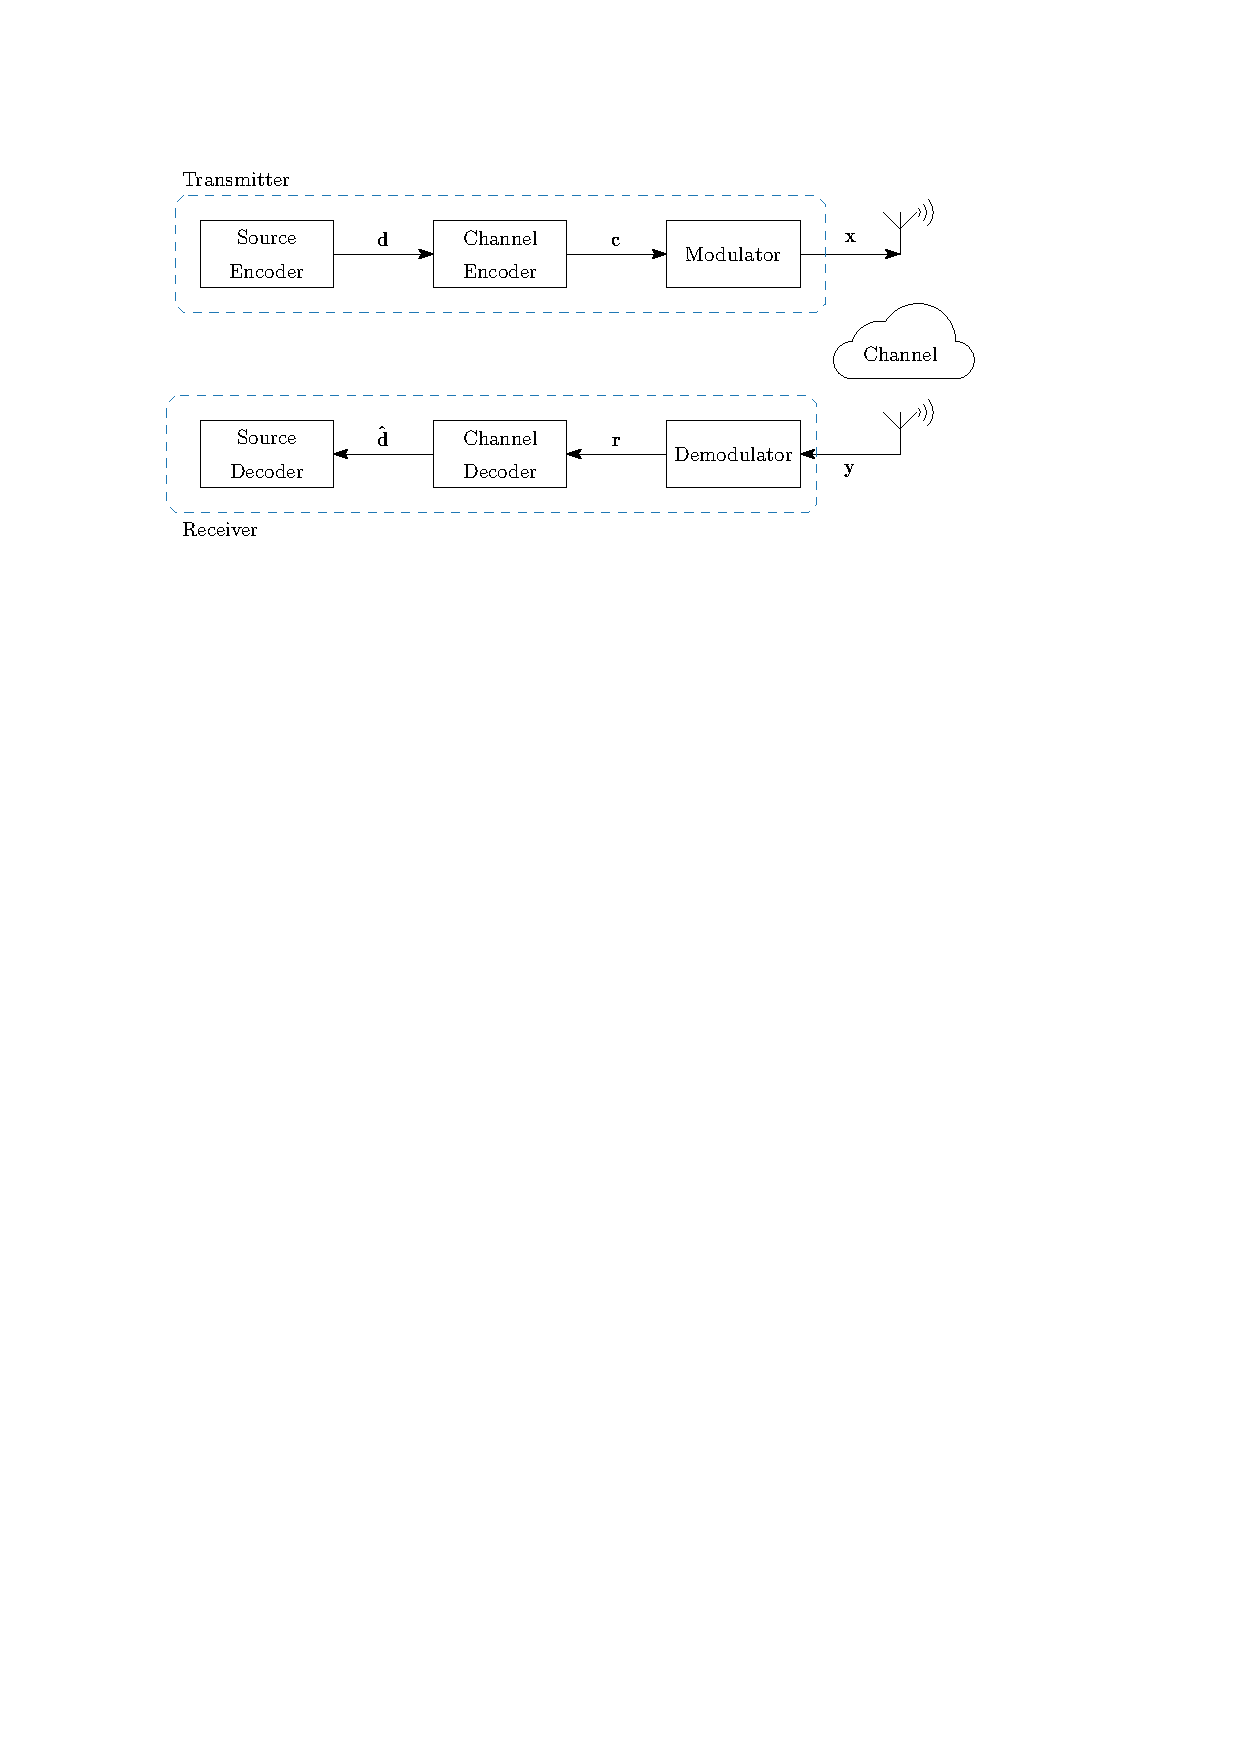
\includegraphics[width=.8\textwidth, page=1]{fig/shParadigm2.pdf}}
    \only<2->{\includegraphics[width=.8\textwidth, page=2]{fig/shParadigm2.pdf}}
  \end{center}
  \vspace*{-1em}
  \begin{itemize}\itmsp{.5em}
    \item<2-> L'un des codes correcteur d'erreurs les plus efficace.
    \item<3> Excellent compromis entre complexité calculatoire et performances de décodage.
    \item<3> Choisis dans plusieurs standards de communication numérique sans-fil :
          \begin{itemize}
            \item Contexte satellitaire (CCSDS, DVB-RCS)
            \item Contexte mobile (LTE)
          \end{itemize}
  \end{itemize}
\end{frame}

\begin{frame}[c]{Turbo codeur}
  \begin{center}
    \only<1>{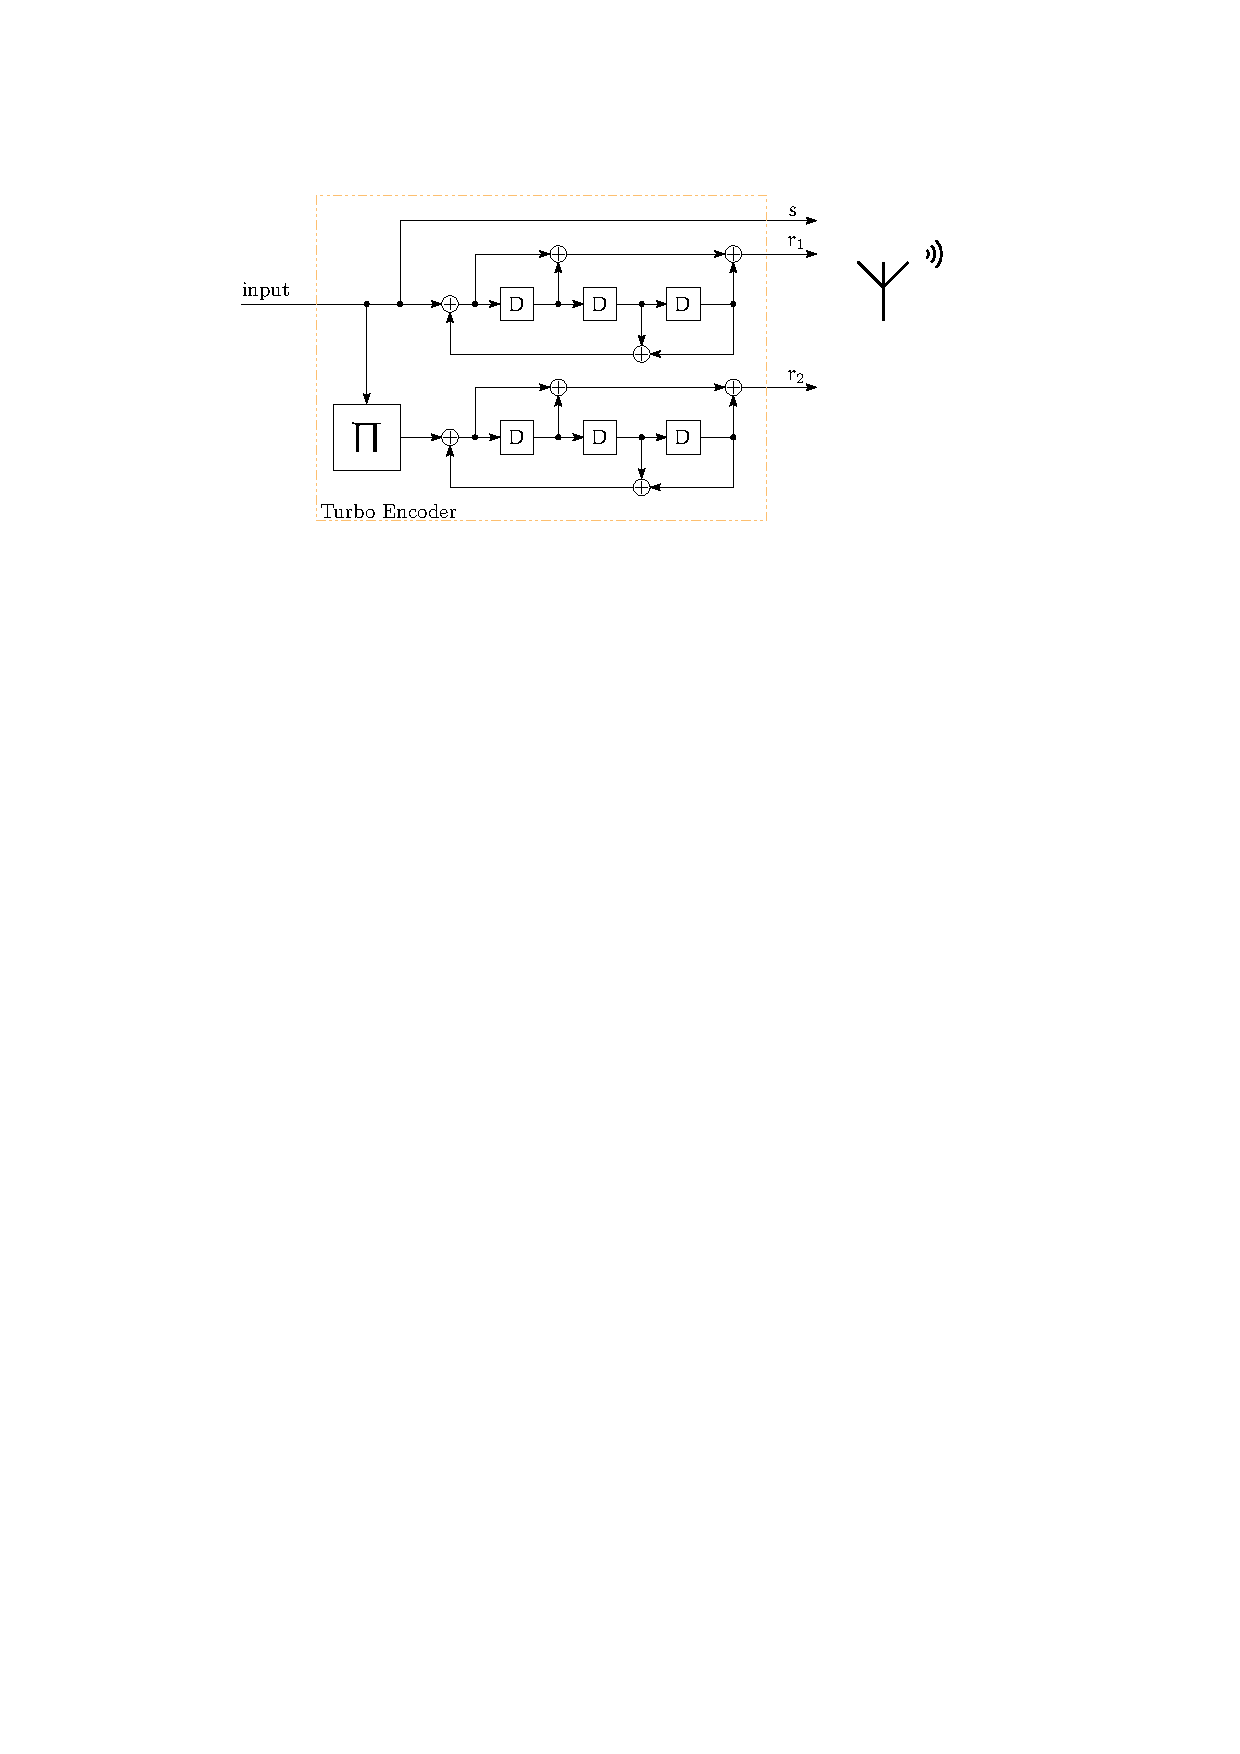
\includegraphics[width=.8\textwidth,page=1]{fig/encoder.pdf}}
    \only<2>{\includegraphics[width=.8\textwidth,page=2]{fig/encoder.pdf}}
    \only<3>{\includegraphics[width=.8\textwidth,page=3]{fig/encoder.pdf}}
  \end{center} 
  \begin{itemize}\itmsp{.5em}
    \item Trois blocs élémentaires : 2 RSC + Entrelaceur
    \item Rendement natif : 1/3
  \end{itemize}
\end{frame}

\begin{frame}[c]{Turbo décodeur}
\begin{overlayarea}{\textwidth}{\textheight}
    \only<1>{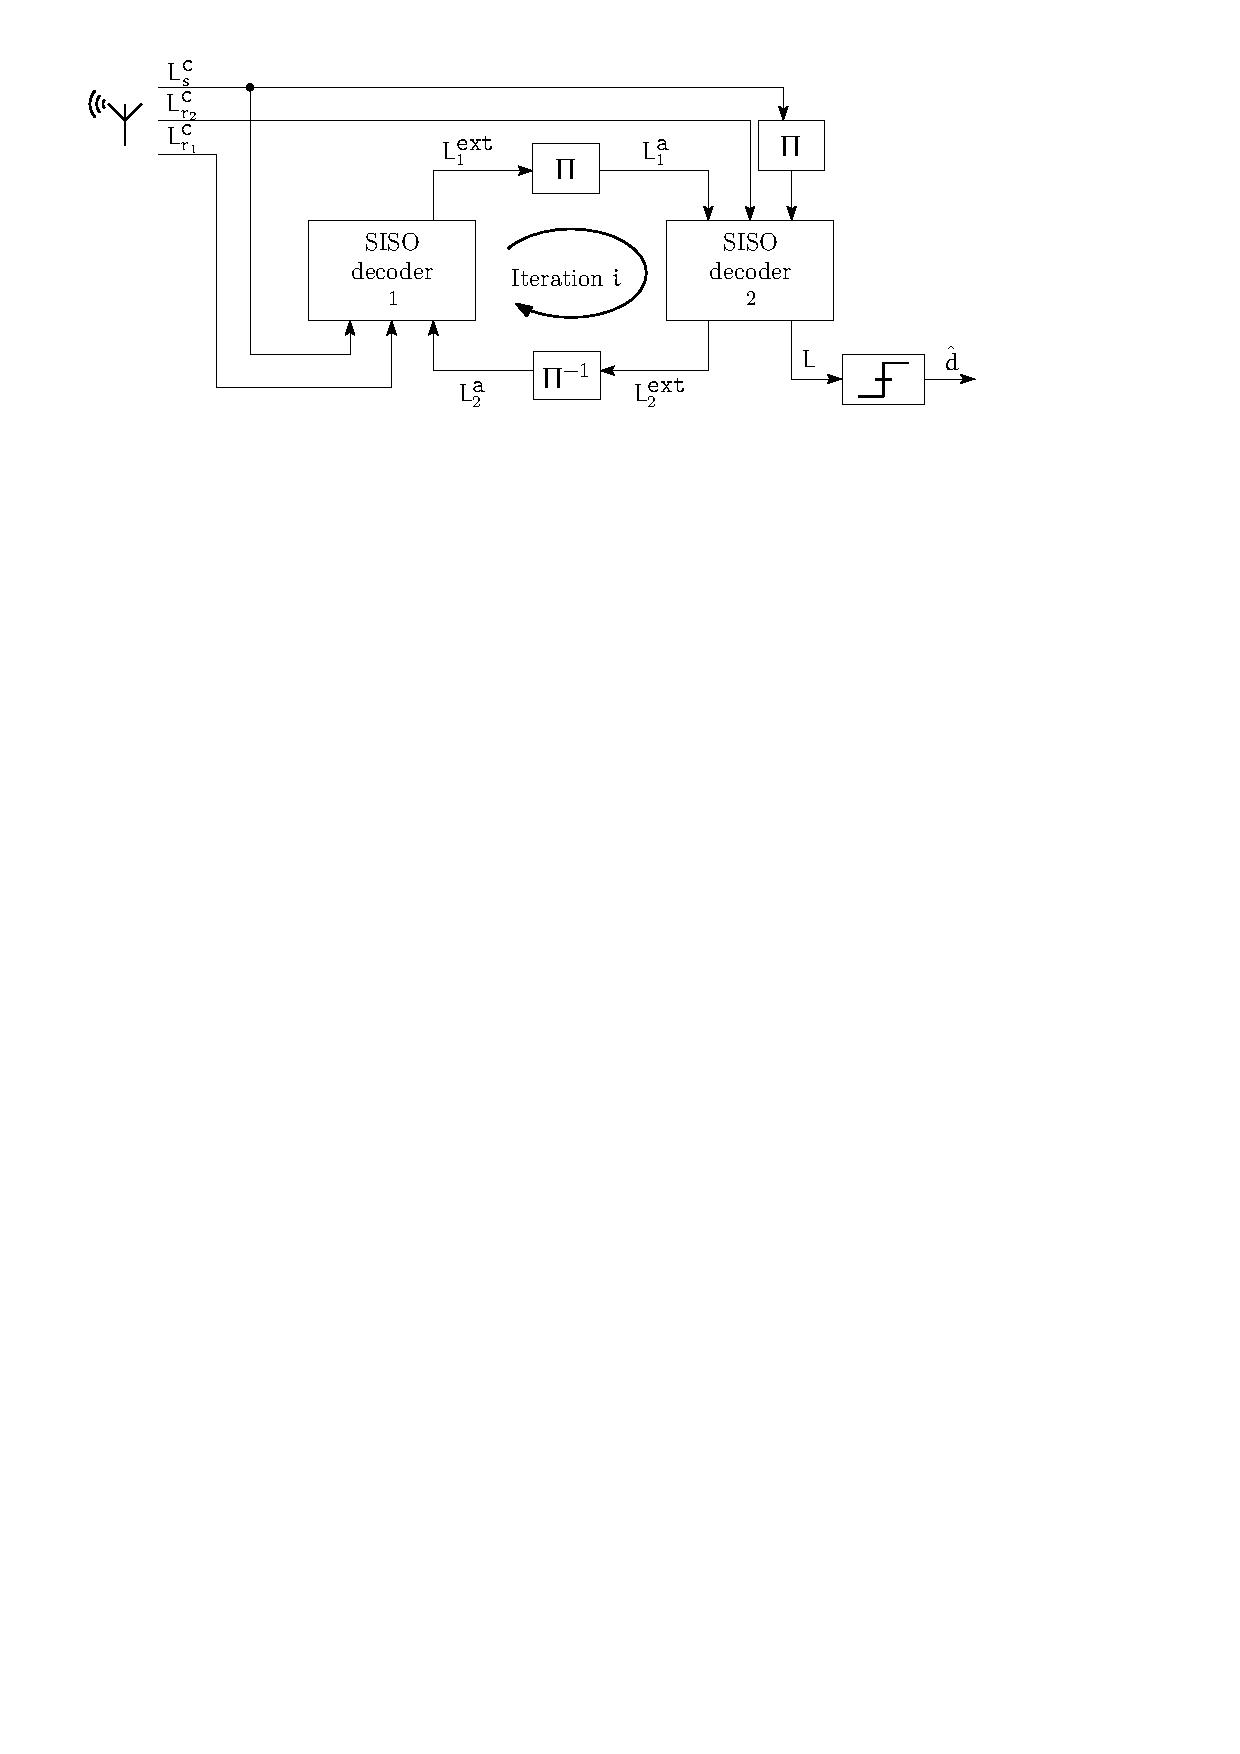
\includegraphics[width=.7\textwidth,page=1, center]{fig/tdec.pdf}}
    \only<2>{\includegraphics[width=.7\textwidth,page=2, center]{fig/tdec.pdf}}
    \only<3>{\includegraphics[width=.7\textwidth,page=3, center]{fig/tdec.pdf}}
    \only<4>{\includegraphics[width=.7\textwidth,page=4, center]{fig/tdec.pdf}}
    \only<5>{\includegraphics[width=.7\textwidth,page=3, center]{fig/tdec.pdf}}
    \only<6>{\includegraphics[width=.7\textwidth,page=5, center]{fig/tdec.pdf}}
  \begin{itemize}\itmsp{.5em}
  \only<1-5>{\vspace*{-1.2em}}
    \item Processus itératif.
    \item 2 SISOs s'échangent leur avis vis l'information extrinsèque ($\mathbf{L^{e}}$).
  \end{itemize}
\end{overlayarea}
\end{frame}

\begin{frame}[c]{Décodeur SISO}
\begin{overlayarea}{\textwidth}{\textheight}
    \only<1>{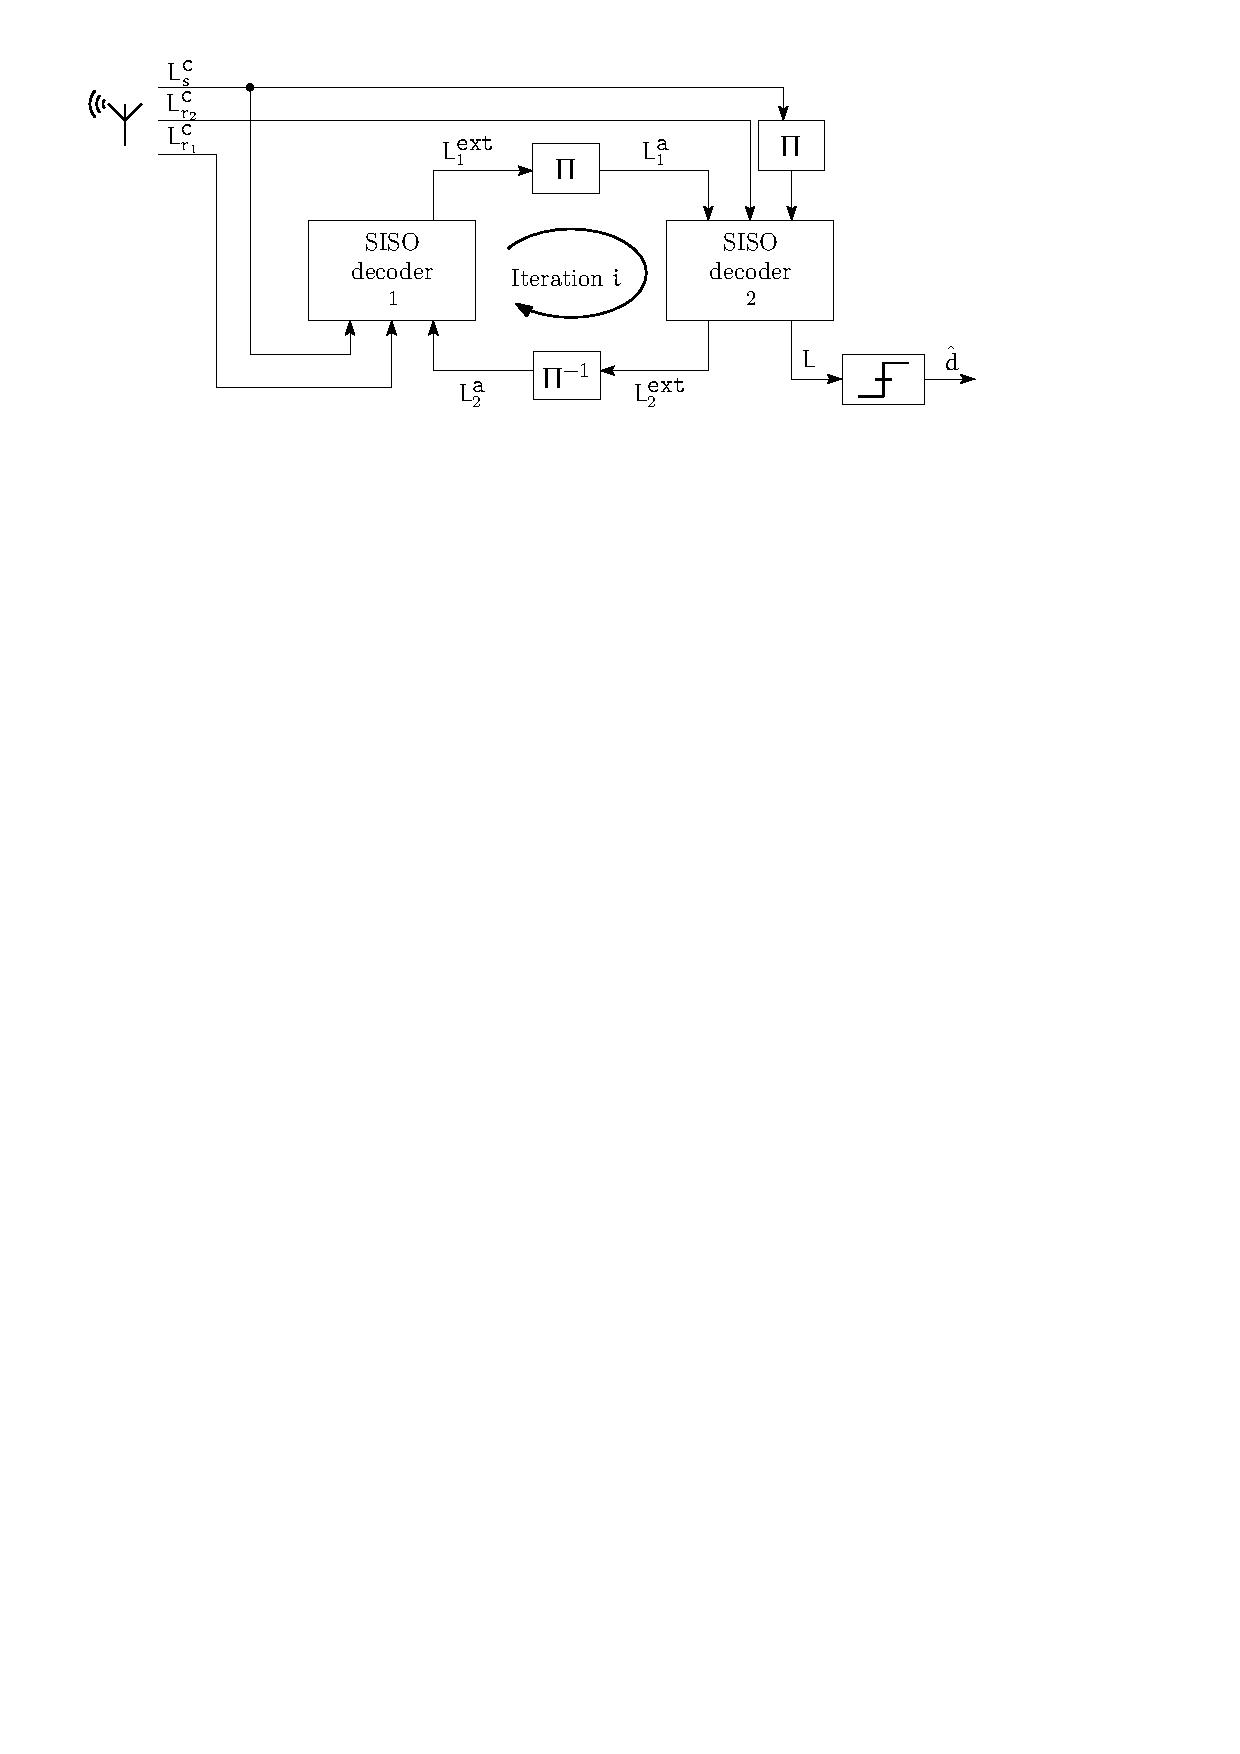
\includegraphics[width=.7\textwidth,page=1, center]{fig/tdec.pdf}}
    \only<2>{\includegraphics[width=.7\textwidth,page=2, center]{fig/tdec.pdf}}
    \only<3>{\includegraphics[width=.7\textwidth,page=3, center]{fig/tdec.pdf}}
    \only<4>{\includegraphics[width=.7\textwidth,page=4, center]{fig/tdec.pdf}}
    \only<5>{\includegraphics[width=.7\textwidth,page=3, center]{fig/tdec.pdf}}
    \only<6>{\includegraphics[width=.7\textwidth,page=5, center]{fig/tdec.pdf}}
  \begin{itemize}\itmsp{.5em}
  \only<1-5>{\vspace*{-1.2em}}
    \item Processus itératif.
    \item Information extrinsèque ($\mathbf{L^{e}}$) échangée à travers étapes entrelacement/désentrelacement.
  \end{itemize}
\end{overlayarea}
\end{frame}

\begin{frame}[c]{La problématique du plancher d'erreurs}
\begin{columns}[T] % align columns
\begin{column}{.48\textwidth}
\begin{center}
\vspace*{-1.5em}
  \begin{tikzpicture}
  \begin{semilogyaxis}[footnotesize, width=\linewidth, height=1.3\linewidth,
      xmin=0, xmax=2.2, xtick={0,0.4,...,2.2},
      %ymin=2e-6,  ymax=0.11,
      xlabel=$E_b/N_0 \text{(dB)}$, ylabel=FER,  grid=both, grid style={gray!30},
     tick align=outside, tickpos=left, legend pos=north east]
                                                                       
      \addplot[mark=o,Paired-5]  table [x=SNR, y=FER] {../main/ch1_fig/std/lte13_2048.dat};                            
      \addplot[Paired-6]  table [x=SNR, y=FER] {../main/ch1_fig/std/lte13_2048_ubound.dat}; 
                                                                                                
     \legend{TC, Borne de l'union}
                                                                                                
  \end{semilogyaxis}
\end{tikzpicture}
%\captionof{figure}{\small Standard LTE, R=1/3, K=2048, Canal AWGN, 8 itérations EML-MAP, borne de l'union}
\end{center}
\end{column}%
\hfill%
\begin{column}{.48\textwidth}
\vspace*{2em}
$\color{bleuUni}\bullet$ Manifestation :\\
La courbe de performances s’aplatit à fort SNR

\vspace*{1em}
$\color{bleuUni}\bullet$ Cause : \\
Distribution de mots de code possédant un faible poids ($d_\text{min}$)

\vspace*{1em}
$\color{bleuUni}\bullet$ Propriété : \\
Erreurs résiduelles en sont responsables (faible BE/FE)
\end{column}%
\end{columns}
\end{frame}

\begin{frame}[c]{Quelles solutions ?}
\begin{enumerate}
  \item \only<2->{\sout}{Modifier le code}
  \begin{itemize}
    \item<1> Entrelaceur,
    \item<1> Nombre d'états du codeur,
    \item<1> Concaténation (BCH, RSC-1 par exemple).
  \end{itemize}
  \item<3-> Modifier l'algorithme de décodage
  \begin{itemize}
    \item<4-> Modifier la transmission de l'information extrinsèque
    \item<5-> Exploiter un code CRC présent dans la majorité des standards
    \item<6> État de l'art :
    \begin{itemize}
      \item<6> Décodage par liste,
      \item<6> Ordered Statistic Decoding,
      \item<6> Décodages multiples d'une même trame.
    \end{itemize}
  \end{itemize}
\end{enumerate}

\end{frame}

%%%%%%%%%%%%%%%%%%%%%%%%%%%%%%%%%%%%%%%% 
\subsection{Conclusion et problématique}

\begin{frame}[c]{Conclusion}
\begin{itemize}\setlength\itemsep{2em}
  \item Notions de codage de canal
  \item Construction et décodage des turbo codes convolutifs
  \item Problème du plancher d'erreurs
\end{itemize}
\end{frame}

\begin{frame}[c]{Problématique}
  \begin{itemize}\setlength\itemsep{2em}
    \item Proposer une amélioration des performances de décodage des turbo codes
    \item Sans modifier le schéma de codage, pour être adapté aux turbo codes standardisés
  \end{itemize}
\end{frame}



%%%%%%%%%%%%%%%%%%%%%%%%%%%%%%%%%%%%%%%%%%%%%%%%%%%%%%%%%%%%%%%%%%%%%%%%%%%%%%%%
\section[Erreurs résiduelles]{Erreurs résiduelles : identification et correction}
%%%%%%%%%%%%%%%%%%%%%%%%%%%%%%%%%%%%%%%%
\subsection{Observations}

\begin{frame}[c]{Exemple standard LTE, K=2048, R=1/3 - BE/FE}
\begin{columns}[T] % align columns
  \begin{column}{.48\textwidth}
    %\begin{center}
    \begin{tikzpicture}
      \begin{semilogyaxis}[footnotesize, width=\linewidth, height=1.3\linewidth,
                          xmin=0, xmax=2.2, xtick={0,0.4,...,2.2},
                          %ymin=2e-6,  ymax=0.11,
                          xlabel=$E_b/N_0 \text{(dB)}$, ylabel=FER,  grid=both, grid style={gray!30},
                          tick align=outside, tickpos=left, legend pos=north east]
                                                                     
        \addplot[mark=o,Paired-5]  table [x=SNR, y=FER] {../main/ch1_fig/std/lte13_2048.dat};                            
                                                                                                       
        \legend{TC}                                                                                        
      \end{semilogyaxis}
    \end{tikzpicture}
    %\end{center}
  \end{column}%
  \hfill%
  \begin{column}{.48\textwidth}
  %\begin{center}
    \begin{tikzpicture}
      \begin{axis}[footnotesize, width=\linewidth, height=1.3\linewidth,
                   xmin=0, xmax=2.2, xtick={0,0.4,...,2.2},
                   ymin=0,  ymax=300,
                    xlabel=$E_b/N_0 \text{(dB)}$, ylabel=BE/FE,  grid=both, grid style={gray!30},
                    tick align=outside, tickpos=left, legend pos=north east]
                                                                       
          \addplot[mark=o,Paired-5, visible on=<2>]  coordinates  {(0.0, 286)  (0.1, 218)  (0.2, 199) (0.3, 112) (0.4, 92) (0.5, 79) (0.6, 77) (0.7, 59) (0.8, 57) 
                                                                   (0.9, 42.6) (1.0, 16.3) (1.1, 4.4) (1.2, 2.8)};
                                                                                                         
          \legend{TC}                                                                                        
      \end{axis}
    \end{tikzpicture}
    %\end{center}
  \end{column}%
\end{columns}
\end{frame}


\begin{frame}[c]{Exemple standard LTE, K=2048, R=1/3 - Fonction de masse}
\begin{center}
   \begin{tikzpicture}
     \begin{axis}[footnotesize, 
           height=.5\textwidth,  width=.9\textwidth,
           grid=both, grid style={gray!30},
           %colorbrewer cycle list=Spectral,
           ybar interval=1pt, %/pgf/bar width=3pt,
           xmin=1, xmax=22, xtick={1,2,...,22}, ymin=0,  ytick={0,10,...,45}, ymax=45, 
           grid=both, grid style={dashed, gray!50},  legend style={at={(0.5,1.03)},anchor=south},legend columns=4,
           xticklabels={1,2,3,4,5,6,7,8,9,10,11,12,13,14,15,16,17,18,19,20,>20},
           x tick label style={shift={(axis cs:1.25,0)},anchor=east,rotate=60},
           restrict y to domain*=0:45, % Cut values off at 14
           visualization depends on=rawy\as\rawy, % Save the unclipped values
           after end axis/.code={\draw [ultra thick, white, decoration={snake, amplitude=1pt}, decorate] (rel axis cs:0,0.95) -- (rel axis cs:1,0.95);},
           axis lines*=left,
           clip=false,
           xlabel = Erreurs binaires,
           ylabel = FdM (\%),
           legend style={at={(0.5,1.03)},anchor=south}, legend columns=4,
           ]
   
          \addplot[draw=Paired-1, fill=Paired-1!50, postaction={pattern color = black!80,pattern=north west lines}, visible on=<2->] table [x=X, y expr=\thisrowno{5}/5] {../main/ch3_fig/be/dat/2048.dat};
          \addplot[draw=Paired-3, fill=Paired-3!50, postaction={pattern color = black!80,pattern=north east lines}, visible on=<3->] table [x=X, y expr=\thisrowno{6}/5] {../main/ch3_fig/be/dat/2048.dat};
          \addplot[draw=Paired-5, fill=Paired-5!50, postaction={pattern color = black!80,pattern=crosshatch dots }, visible on=<4->] table [x=X, y expr=\thisrowno{7}/5] {../main/ch3_fig/be/dat/2048.dat};
          \addplot[mark=*, only marks, black, mark options={scale=0.9, fill=Dark2-2!50 }, update limits=false, visible on=<5->] table[x=X, y=l2048] {../main/ch3_fig/be/dat/th};

          \legend{$0.9$ dB,$1.1$ dB,$1.3$ dB, Théorique $1.3$ dB}

          \end{axis}
   \end{tikzpicture}
\end{center}
\end{frame}

\begin{frame}[c]{Analyse}
  \begin{enumerate}\setlength\itemsep{1em}
    \item Dans la zone de convergence, de nombreuses erreurs sont présentes à l’issu du décodage. 
    \item En revanche, dans la zone du plancher d’erreurs, le nombre moyen d’erreurs binaires par trame erronée est inférieur à 10. 
    \item La zone du plancher d'erreur émane de la présence \emph{d'erreurs résiduelles}
    \item Le nombre d'erreurs binaires par trame peut être caractérisé grâce au spectre de distance
  \end{enumerate}
\end{frame}

%%%%%%%%%%%%%%%%%%%%%%%%%%%%%%%%%%%%%%%%
\subsection{Critères d'identifications de positions erronés}
\begin{frame}[c]{Le critère}
\begin{itemize}\setlength\itemsep{1em}
  \item Suite à une étude : $    \Delta(k) = |L(k)|, \qquad \text{avec k~}\in \llbracket0;~K \rrbracket $
  \item Module de l'information \textit{a posteriori} {\color{bleuUni}\Large\MVRightarrow} niveau de confiance associé à chaque bit du
mot décodé.
\end{itemize}
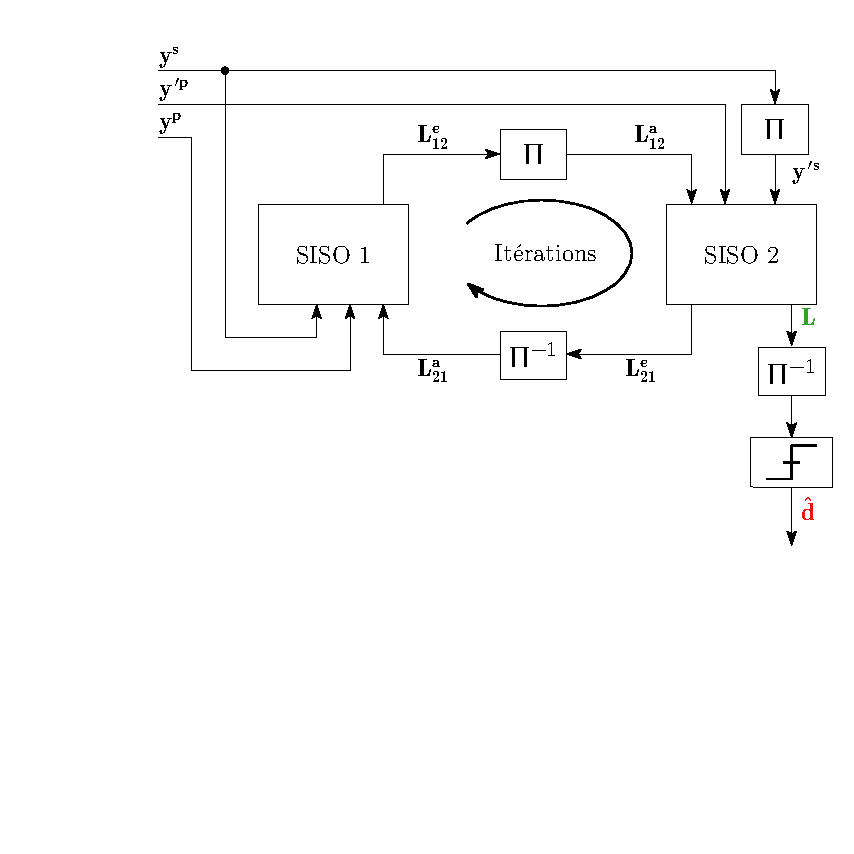
\includegraphics[width=.7\textwidth,page=1, center]{fig/delta.pdf}
\end{frame}

\begin{frame}[c]{Résultats d'identification}
\begin{columns}[T] % align columns
  \begin{column}{.48\textwidth}
  \begin{tikzpicture}
    \begin{axis}[
    height=.8\textheight,  width=\textwidth,
          grid=both, grid style={gray!30},
          %colorbrewer cycle list=Spectral,
          ybar interval = 1pt, /pgf/bar width=-5pt,
          xmin=1, xmax=6, ymin=0,  ytick={0,10,...,105}, ymax=105, 
          grid=both, grid style={dashed, gray!50},  legend style={at={(0.5,1.05)},anchor=south},legend columns=4,
          xticklabels={4, 6, 8, 10, 20},
          ylabel=Identification réussie (\%),
          x tick label style={shift={(axis cs:1.15,-2.5)},anchor=east},  
          axis lines*=left,
          xlabel=Profondeur de recherche,
          legend entries = {Métrique $\Delta$}
          %legend entries = {Métrique Apost.~~, Métrique Ext.~~}
          ]
         
        \only<2>{\addplot[draw=marronUni!50!black, fill=bleuUni!50] table [x=X, y expr=\thisrowno{2}/5.0, restrict x to domain=0:2] {../main/ch3_fig/id2/dat/2048};}
        % \only<3>{\addplot[draw=marronUni!50!black, fill=bleuUni!50, restrict x to domain=0:3] table [x=X, y expr=\thisrowno{2}/5.0] {../main/ch3_fig/id2/dat/2048};}
        % \only<4>{\addplot[draw=marronUni!50!black, fill=bleuUni!50, restrict x to domain=0:4] table [x=X, y expr=\thisrowno{2}/5.0] {../main/ch3_fig/id2/dat/2048};}
        % \only<5>{\addplot[draw=marronUni!50!black, fill=bleuUni!50, restrict x to domain=0:5] table [x=X, y expr=\thisrowno{2}/5.0] {../main/ch3_fig/id2/dat/2048};}
        % \only<6>{\addplot[draw=marronUni!50!black, fill=bleuUni!50, restrict x to domain=0:6] table [x=X, y expr=\thisrowno{2}/5.0] {../main/ch3_fig/id2/dat/2048};}

%        \only<2>{\addplot[draw=marronUni!50!black, fill=bleuUni!50] table [x=X, y expr=\thisrowno{4}/5.0] {../main/ch3_fig/id2/dat/2048};}

 %       \only<3>{\addplot[draw=marronUni!50!black, fill=bleuUni!50] table [x=X, y expr=\thisrowno{6}/5.0] {../main/ch3_fig/id2/dat/2048};}
   
    \end{axis}
    % \only<1>{\node[below = 1cm of be c1r1.south] {(a) : LTE K=2048, SNR=0.9dB (TET=$1.3\times 10^{-4}$)};}
    % \only<2>{\node[below = 1cm of be c1r1.south] {(a) : LTE K=2048, SNR=1.1dB (TET=$1.0\times 10^{-5}$)};}
    % \only<3>{\node[below = 1cm of be c1r1.south] {(a) : LTE K=2048, SNR=1.3dB (TET=$4.3\times 10^{-6}$)};}
    % \only<1>{\node[below = 1cm of be c2r1.south] {(b) : LTE K=6144, SNR=0.4dB (TET=$1.4\times 10^{-1}$)};}
    % \only<2>{\node[below = 1cm of be c2r1.south] {(b) : LTE K=6144, SNR=0.6dB (TET=$1.3\times 10^{-3}$)};}
    % \only<3>{\node[below = 1cm of be c2r1.south] {(b) : LTE K=6144, SNR=0.8dB (TET=$3.4\times 10^{-5}$)};}
  \end{tikzpicture}
  \end{column}%
  \hfill%
  \begin{column}{.48\textwidth}
   \begin{tikzpicture}
     \begin{axis}[footnotesize, 
           height=.6\textwidth,  width=\textwidth,
           grid=both, grid style={gray!30},
           %colorbrewer cycle list=Spectral,
           ybar interval=1pt, %/pgf/bar width=3pt,
           xmin=1, xmax=11, xtick={1,2,...,11}, ymin=0,  ytick={0,10,...,45}, ymax=45, 
           grid=both, grid style={dashed, gray!50},  legend style={at={(0.5,1.03)},anchor=south},legend columns=4,
           xticklabels={1,2,3,4,5,6,7,8,9,10},
           x tick label style={shift={(axis cs:1.25,0)},anchor=east,rotate=60},
           restrict y to domain*=0:45, % Cut values off at 14
           visualization depends on=rawy\as\rawy, % Save the unclipped values
           after end axis/.code={\draw [ultra thick, white, decoration={snake, amplitude=1pt}, decorate] (rel axis cs:0,0.95) -- (rel axis cs:1,0.95);},
           axis lines*=left,
           clip=false,
           xlabel = Erreurs binaires,
           ylabel = FdM (\%),
           legend style={at={(0.5,1.03)},anchor=south}, legend columns=4,
           ]
   
          \addplot[draw=Paired-1, fill=Paired-1!50, postaction={pattern color = black!80,pattern=north west lines}, visible on=<2->, restrict x to domain=1:11] table [x=X, y expr=\thisrowno{5}/5] {../main/ch3_fig/be/dat/2048.dat};
          \addplot[draw=Paired-3, fill=Paired-3!50, postaction={pattern color = black!80,pattern=north east lines}, visible on=<3->, restrict x to domain=1:11] table [x=X, y expr=\thisrowno{6}/5] {../main/ch3_fig/be/dat/2048.dat};
          \addplot[draw=Paired-5, fill=Paired-5!50, postaction={pattern color = black!80,pattern=crosshatch dots }, visible on=<4->, restrict x to domain=1:11] table [x=X, y expr=\thisrowno{7}/5] {../main/ch3_fig/be/dat/2048.dat};
          %\addplot[mark=*, only marks, black, mark options={scale=0.9, fill=Dark2-2!50 }, update limits=false, visible on=<5->] table[x=X, y=l2048] {../main/ch3_fig/be/dat/th};

          \legend{$0.9$ dB,$1.1$ dB,$1.3$ dB}%, Théorique $1.3$ dB}

          \end{axis}
   \end{tikzpicture}

    \end{column}%
\end{columns}

\end{frame}

%%%%%%%%%%%%%%%%%%%%%%%%%%%%%%%%%%%%%%%%
\subsection{L'algorithme FNC}

%%%%%%%%%%%%%%%%%%%%%%%%%%%%%%%%%%%%%%%%%%%%%%%%%%%%%%%%%%%%%%%%%%%%%%%%%%%%%%%%
\section[Architecture matérielle]{Architecture matérielle de correction des erreurs résiduelles}
%%%%%%%%%%%%%%%%%%%%%%%%%%%%%%%%%%%%%%%%
\subsection{Implantation matérielle de turbo décodeurs}


%%%%%%%%%%%%%%%%%%%%%%%%%%%%%%%%%%%%%%%%
\subsection{Les paramètres de l'algorithme FNC}

%%%%%%%%%%%%%%%%%%%%%%%%%%%%%%%%%%%%%%%%
\subsection{Implantation matérielle de l'algorithme FNC}


%%%%%%%%%%%%%%%%%%%%%%%%%%%%%%%%%%%%%%%%%%%%%%%%%%%%%%%%%%%%%%%%%%%%%%%%%%%%%%%%
\section[Conclusions]{Conclusions et perspectives}

\begin{frame}[c]{Conclusions}
TODO
\end{frame}

\begin{frame}[c]{Perspectives}
TODO
\end{frame}

\begin{frame}[c]{Merci}
\begin{center}
Merci pour votre attention !
\end{center}
\end{frame}

\end{document}
